\documentclass[11pt]{article}
\usepackage[utf8]{inputenc}
\usepackage{natbib}
\usepackage{graphicx}
\usepackage{url}
\usepackage{amsmath, amssymb}
\usepackage[margin=1in]{geometry}
\usepackage{setspace}
\usepackage{enumitem}
\usepackage{booktabs}
\usepackage{float}
\usepackage{needspace}

% Formatting
\setstretch{1.2}

% ============================================================
% EASY-TO-UPDATE STATISTICS
% After running code/eda_analysis_regression.py, replace these values
% with the numbers printed to the console.
% ============================================================
\newcommand{\totalRaw}{711{,}897}        % raw pitches before cleaning
\newcommand{\totalPitches}{702{,}321}    % pitches after cleaning
\newcommand{\overallWhiff}{12.0}         % overall whiff rate (%)
\newcommand{\numBatters}{531}            % unique batters (>= 200 pitches)
\newcommand{\numPitchers}{811}           % unique pitchers
\newcommand{\batterLow}{2.4}             % lowest batter whiff rate (%)
\newcommand{\batterHigh}{23.2}           % highest batter whiff rate (%)

% ============================================================
% FINAL REPORT MODEL RESULTS
% After running code/eda_analysis_regression.py, code/combined_model.R,
% and the notebook in code/eda_regression.ipynb, replace these values
% with the printed model summaries.
% ============================================================
\newcommand{\seqLLBase}{-203{,}264.99}
\newcommand{\seqLLSeq}{-200{,}685.21}
\newcommand{\seqLRStat}{5{,}159.56}
\newcommand{\seqLRDf}{91}
\newcommand{\seqLRPval}{$< 10^{-16}$}
\newcommand{\seqBICBase}{406{,}595.79}
\newcommand{\seqBICSeq}{402{,}634.04}
\newcommand{\seqDeltaBIC}{-3{,}961.76}
\newcommand{\glmmObs}{30{,}000}
\newcommand{\glmmBatters}{649}
\newcommand{\glmmFixed}{96}
\newcommand{\glmmSigma}{0.301}
\newcommand{\glmmSigmaSq}{0.091}
\newcommand{\glmmICC}{2.69}
\newcommand{\combLogLik}{-198{,}638.43}
\newcommand{\combBIC}{398{,}487.82}
\newcommand{\combRandSD}{0.327}
% ============================================================

\title{\textbf{Modeling the Effect of Pitch Sequencing and\\
Batter-Specific Adjustments on Swing-and-Miss\\
Outcomes in MLB} \\[6pt]
\large Final Project Report}
\author{Group 10: Harsh Dave, Nick Griffin, Jack Leidlein, Hector Carrillo}
\date{Spring 2026}

\begin{document}
\maketitle

%%==============================================================
\section{Introduction}
%%==============================================================

The introduction of the Statcast tracking system in Major League Baseball (MLB) in 2015 fundamentally changed how teams evaluate pitching performance.
Every pitch thrown in an MLB game is now measured across dozens of metrics---release speed, spin rate, movement profile, release point, and extension---captured at the millisecond level \citep{statcast2024}.
This wealth of data has fueled a shift in pitcher development strategy, with front offices increasingly investing in data-driven approaches to maximize the effectiveness of each pitch in a pitcher's arsenal.

At the core of modern pitching analytics lies a central question: \textit{what attributes make a pitch difficult to hit?}
Intuitively, pitches with higher velocity, greater movement, and longer extension should be harder to contact.
However, standard logistic regression models that predict swing-and-miss (whiff) probability based solely on these physical characteristics often produce inconclusive results.
In such models, the probability of a whiff, $p_i = P(Y_i = 1)$, is typically modeled as:
%
\begin{equation}\label{eq:baseline}
    \log\!\left(\frac{p_i}{1 - p_i}\right)
    = \beta_0
    + \beta_1 \,\texttt{Speed}_i
    + \beta_2 \,\texttt{IVB}_i
    + \beta_3 \,\texttt{HB}_i
    + \beta_4 \,\texttt{Ext}_i
\end{equation}
%
where \texttt{IVB} denotes induced vertical break, \texttt{HB} horizontal break, and \texttt{Ext} release extension.
This four-variable baseline is the physical-characteristics specification used throughout the report; arm angle is not included as a separate model term because the cleaned modeling matrix retains release speed, IVB, HB, and release extension as the consistent pitch-level physical measures.
Previous studies using this framework have found that main effects and simple interactions are often statistically insignificant or fail to explain the observed variation in outcomes.

The fundamental limitation of this approach is that it treats each pitch as an independent, context-free event, ignoring two critical sources of variation: \textbf{sequencing} and \textbf{batter heterogeneity}.
First, pitches are part of a strategic sequence within a plate appearance.
A pitch's effectiveness depends not only on its own physical properties but also on the buildup leading to it.
For example, a slider may induce more whiffs when preceded by a fastball, because the speed differential disrupts the batter's timing---a phenomenon known as pitch tunneling \citep{toporek2017tunneling}.
Second, batters differ substantially in their baseline contact rates.
Elite contact hitters rarely swing and miss regardless of pitch quality, while high-strikeout batters may whiff at average pitches.
Ignoring these batter-specific tendencies introduces unmodeled heterogeneity that weakens inference about the true relationship between pitch quality and outcomes.

To address these limitations, we propose a framework that incorporates both pitch sequencing and batter heterogeneity.
Specifically, our research question is:

\begin{quote}
\centering
\textit{How do pitch sequencing (the type, location, and result of the previous pitch) and batter-specific tendencies jointly influence the probability of a swing-and-miss, beyond the physical characteristics of the pitch itself?}
\end{quote}

\noindent
We pursue three objectives:
\begin{enumerate}[leftmargin=3em, label=\textbf{\arabic*.}]
    \item \textbf{Pitch Sequence Effects:} Investigate whether the previous pitch type and result significantly affect the whiff probability of the current pitch, and identify which sequence combinations (e.g., Fastball $\rightarrow$ Slider) show the largest effects.
    \item \textbf{Batter Skill vs.\ Pitch Quality:} Implement a Generalized Linear Mixed Model (GLMM) with batter random effects to separate variance attributable to the pitch from variance attributable to the batter's contact ability \citep{gelman2006data, bolker2009glmm}.
    \item \textbf{Model Comparison:} Evaluate whether models incorporating sequencing and mixed effects provide better fit and predictive power compared to the baseline physical-characteristics model, using likelihood ratio tests and BIC \citep{mccullagh2019generalized}.
\end{enumerate}

In this report, we describe the dataset, summarize the exploratory patterns that motivate the model structure, and then present results for four complementary models: a baseline logistic regression, a sequencing model, a GLMM with batter random intercepts, and a combined model that incorporates both sequencing and batter heterogeneity.

%%==============================================================
\section{Data Description}
%%==============================================================

\subsection{Data Source and Collection}

Our dataset consists of pitch-level observations from the 2025 MLB regular season, obtained from the Statcast tracking system via the \texttt{pybaseball} Python module \citep{pybaseball}.
Statcast uses a combination of radar and optical tracking to record high-resolution measurements for every pitch thrown in MLB games.
We retrieved approximately \totalRaw{} pitch records spanning the full 2025 regular season (March 27 through September 28), prior to any cleaning or filtering.

\subsection{Unit of Observation and Response Variable}

The unit of observation is an individual pitch.
For each pitch~$i$, we define a binary response variable:
\[
   Y_i =
   \begin{cases}
   1 & \text{if the batter swings and misses (whiff)}, \\
   0 & \text{otherwise}.
   \end{cases}
\]
A whiff is identified using the Statcast \texttt{description} field; specifically, 
we classify a pitch as a whiff when the description is \texttt{swinging\_strike} 
(the batter swings and completely misses the pitch), \texttt{swinging\_strike\_blocked} 
(the batter swings and misses a pitch in the dirt that is blocked by the catcher), 
or \texttt{foul\_tip} (the batter swings and grazes the pitch directly into 
the catcher's mitt for a strike).

\subsection{Predictor Variables}

We organize predictors into three categories:

\medskip
\noindent\textbf{(1) Physical Pitch Characteristics.}
These are the measurable properties of each individual pitch:
\begin{itemize}[nosep]
    \item Release Speed (mph): Velocity of the pitch at the point of release from the pitcher's hand.
    \item Induced Vertical Break (in.): Vertical movement of the pitch relative to a theoretical spinless pitch.
    \item Horizontal Break (in.): Lateral movement of the pitch relative to a theoretical spinless pitch.
    \item Release Extension (ft): Distance from the pitcher's plate to where the pitcher releases the ball.
\end{itemize}

\medskip
\noindent\textbf{(2) Sequencing Variables.}
To capture the strategic context of each pitch, we construct lagged variables within each plate appearance:
\begin{itemize}[nosep]
    \item Previous Pitch Type: Statcast pitch type code of the preceding pitch in the plate appearance (e.g., fastball, slider, changeup).
    \item Previous Pitch Zone: Statcast strike zone region (zones 1--14) in which the preceding pitch was located.
    \item Previous Pitch Outcome: Result of the preceding pitch, categorized as ball, called strike, swinging strike, foul, or in-play.
    \item Pitch Type Interaction: Combination of the previous and current pitch types, used to capture sequence-specific effects.
\end{itemize}
Lag variables are constructed strictly within the same plate appearance.
For the first pitch of an at-bat, previous-pitch fields are coded as a distinct ``None'' category to preserve the observation rather than discard it.

\medskip
\noindent\textbf{(3) Batter-Specific Effects.}
Batters differ substantially in their baseline tendency to swing and miss, independent of pitch quality. 
To account for this contact heterogeneity without estimating \numBatters{} separate fixed coefficients, batter identity will be incorporated as a random effect in the GLMM, 
allowing the model to partially pool information across batters and produce shrinkage estimates for those with limited observations.

\subsection{Data Cleaning}

We apply the following filters to ensure data quality:
\begin{enumerate}[nosep]
    \item \textbf{Remove non-competitive events:} Pitchouts and intentional balls are excluded, as these pitches are not thrown with the intent to retire the batter and would distort whiff rate estimates.
    \item \textbf{Exclude pitches with missing physical measurements:} Pitches with missing physical characteristics such as Release Speed are dropped, as these variables are required predictors in all planned models. 
    \item \textbf{Remove pitches with unrealistic release speeds:} Pitches with a recorded release speed below 65 mph or above 105 mph are removed, as these values fall outside the physically plausible range for MLB pitchers and are indicative of tracking errors.
    \item \textbf{Restrict to nine most common pitch types:} Only the nine most frequently thrown pitch types are retained, ensuring sufficient observations and reliable inference in each category---four-seam fastball (FF), sinker (SI), cutter (FC), slider (SL), sweeper (ST), curveball (CU), knuckle-curve (KC), changeup (CH), and splitter (FS).
\end{enumerate}
After cleaning, our working dataset contains \totalPitches{} pitches with an overall whiff rate of \overallWhiff\%.

%%==============================================================
\section{Exploratory Data Analysis}
%%==============================================================

Before proceeding to formal modeling, we conduct an exploratory analysis to characterize the key patterns in the data and motivate our modeling choices.
All analysis and visualization is performed in Python using the \texttt{matplotlib} \citep{matplotlib2007} and \texttt{seaborn} \citep{seaborn2021} libraries.

\subsection{Summary Statistics}

Table~\ref{tab:summary} presents descriptive statistics for the four primary physical pitch characteristics.
Release speed has a mean of approximately 89.5 mph with a standard deviation of 5.8 mph, which reflects the typical mix of fastballs (mid-to-upper 90s) and off-speed pitches (low-to-mid 80s) in a normal MLB game.
Induced vertical break averages 6.9 inches but spans a wide range ($-$24.0 to 27.5 in.), capturing the contrast between pitches with heavy topspin (negative IVB, such as curveballs) and those with strong backspin (positive IVB, such as four-seam fastballs).
Horizontal break also exhibits substantial variability with a standard deviation of 10.8 inches, reflecting the diversity of pitch types and lateral movement profiles in the dataset.

\begin{table}[H]
\centering
\begin{tabular}{lrrrr}
\toprule
Variable & Mean & SD & Min & Max \\
\midrule
Release Speed (mph)           & 89.5 & 5.8 & 65.2 & 104.2 \\
Induced Vertical Break (in.)  & 6.9 & 8.6 & $-$24.0 & 27.5 \\
Horizontal Break (in.)        & $-$1.6  & 10.8 & $-$29.4 & 30.5 \\
Release Extension (ft)        & 6.4  & 0.4 & 3.9 & 9.6 \\
\bottomrule
\end{tabular}
\caption{Summary statistics for key physical pitch characteristics in the cleaned 2025 dataset.}
\label{tab:summary}
\end{table}

\subsection{Whiff Rates by Pitch Type}

Not all pitch types are equally effective at generating swing-and-miss outcomes.
Figure~\ref{fig:whiff_type} displays the whiff rate for each pitch type in the dataset.
Splitters lead with the highest whiff rate (17.9\%), followed by sliders (16.2\%) and knuckle-curves (16.1\%).
Off-speed and breaking pitches consistently outperform fastball variants: the three highest-whiff-rate pitch types are all non-fastball pitches, while sinkers produce the lowest whiff rate at just 6.3\%.
This pattern is expected, as off-speed and breaking pitches are designed to deceive the batter through movement and speed differential rather than pure velocity.
Table~\ref{tab:whiff_type} provides the corresponding counts.

\begin{figure}[H]
    \centering
    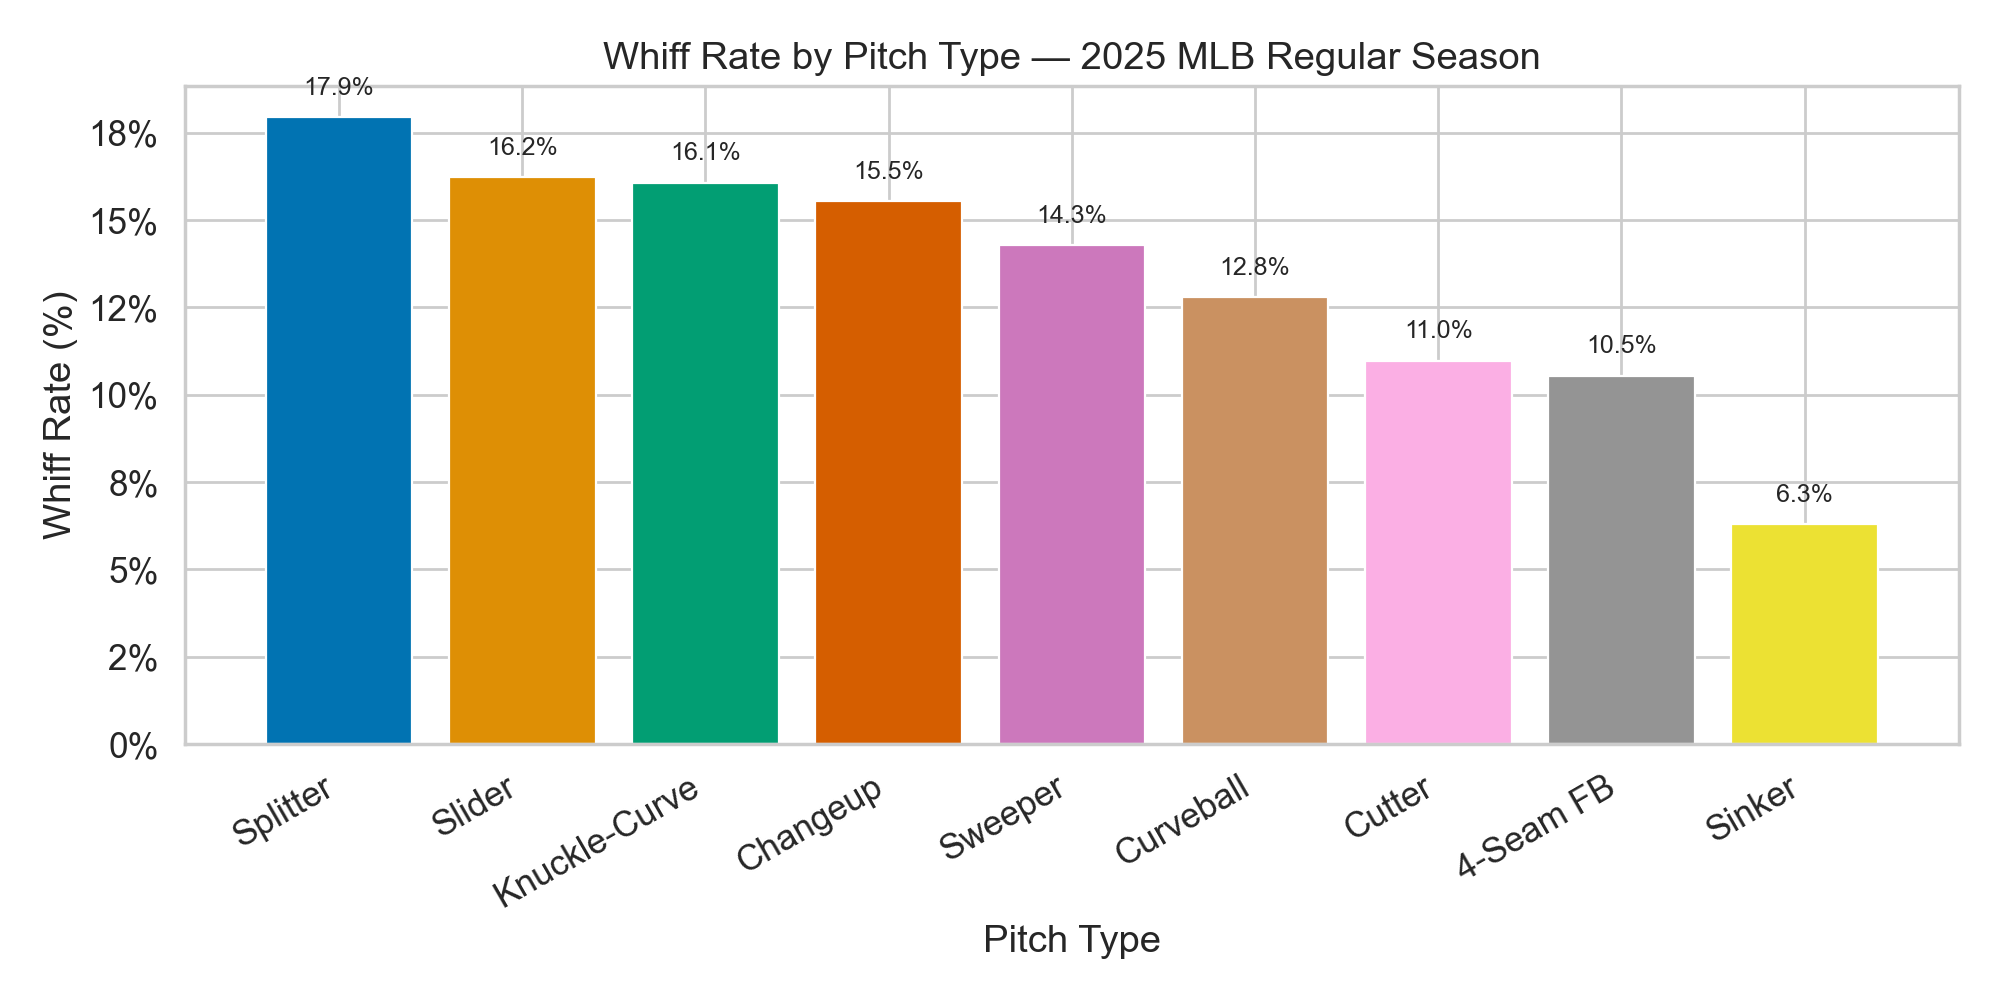
\includegraphics[width=0.85\textwidth]{figures/fig_whiff_by_pitch_type.png}
    \caption{Whiff rate by pitch type in the 2025 MLB regular season. Breaking balls and off-speed pitches consistently show higher whiff rates than fastball variants.}
    \label{fig:whiff_type}
\end{figure}

\begin{table}[H]
\centering
\begin{tabular}{lrrr}
\toprule
Pitch Type & Total Pitches & Whiffs & Whiff Rate (\%) \\
\midrule
Splitter      & 23,155  & 4,154  & 17.9 \\
Slider        & 103,611 & 16,816 & 16.2 \\
Knuckle-Curve & 12,647  & 2,033  & 16.1 \\
Changeup      & 72,959  & 11,337 & 15.5 \\
Sweeper       & 52,305  & 7,472  & 14.3 \\
Curveball     & 47,617  & 6,088  & 12.8 \\
Cutter        & 53,540  & 5,873  & 11.0 \\
4-Seam FB     & 225,924 & 23,820 & 10.5 \\
Sinker        & 110,563 & 6,958  & 6.3 \\
\bottomrule
\end{tabular}
\caption{Whiff rates by pitch type in the 2025 MLB regular season.}
\label{tab:whiff_type}
\end{table}

\subsection{Physical Pitch Characteristic Distributions}

Figure~\ref{fig:phys_dist} compares the distributions for whiff and non-whiff pitches of release speed, induced vertical break, horizontal break, and release extension.
Several patterns emerge.
Pitches that result in whiffs tend to have slightly lower average release speeds. This makes sense because breaking balls and off-speed pitches, which are thrown at lower velocities, generate whiffs at higher rates.
The induced vertical break distribution for whiffs is shifted toward lower (and more negative) values compared to non-whiffs. This also makes sense as pitches with downward break such as sliders, sweepers, and curveballs gnerate more swing-and-misses.
The horizontal break distribution for whiffs shows heavier tails, reflecting the extreme lateral movement of sliders and sweepers.
Release extension distributions are largely overlapping between the two groups.
Overall, these distributional differences, while visible, are not dramatic for any single variable in isolation, which reinforces the need for multivariate modeling.

\begin{figure}[H]
    \centering
    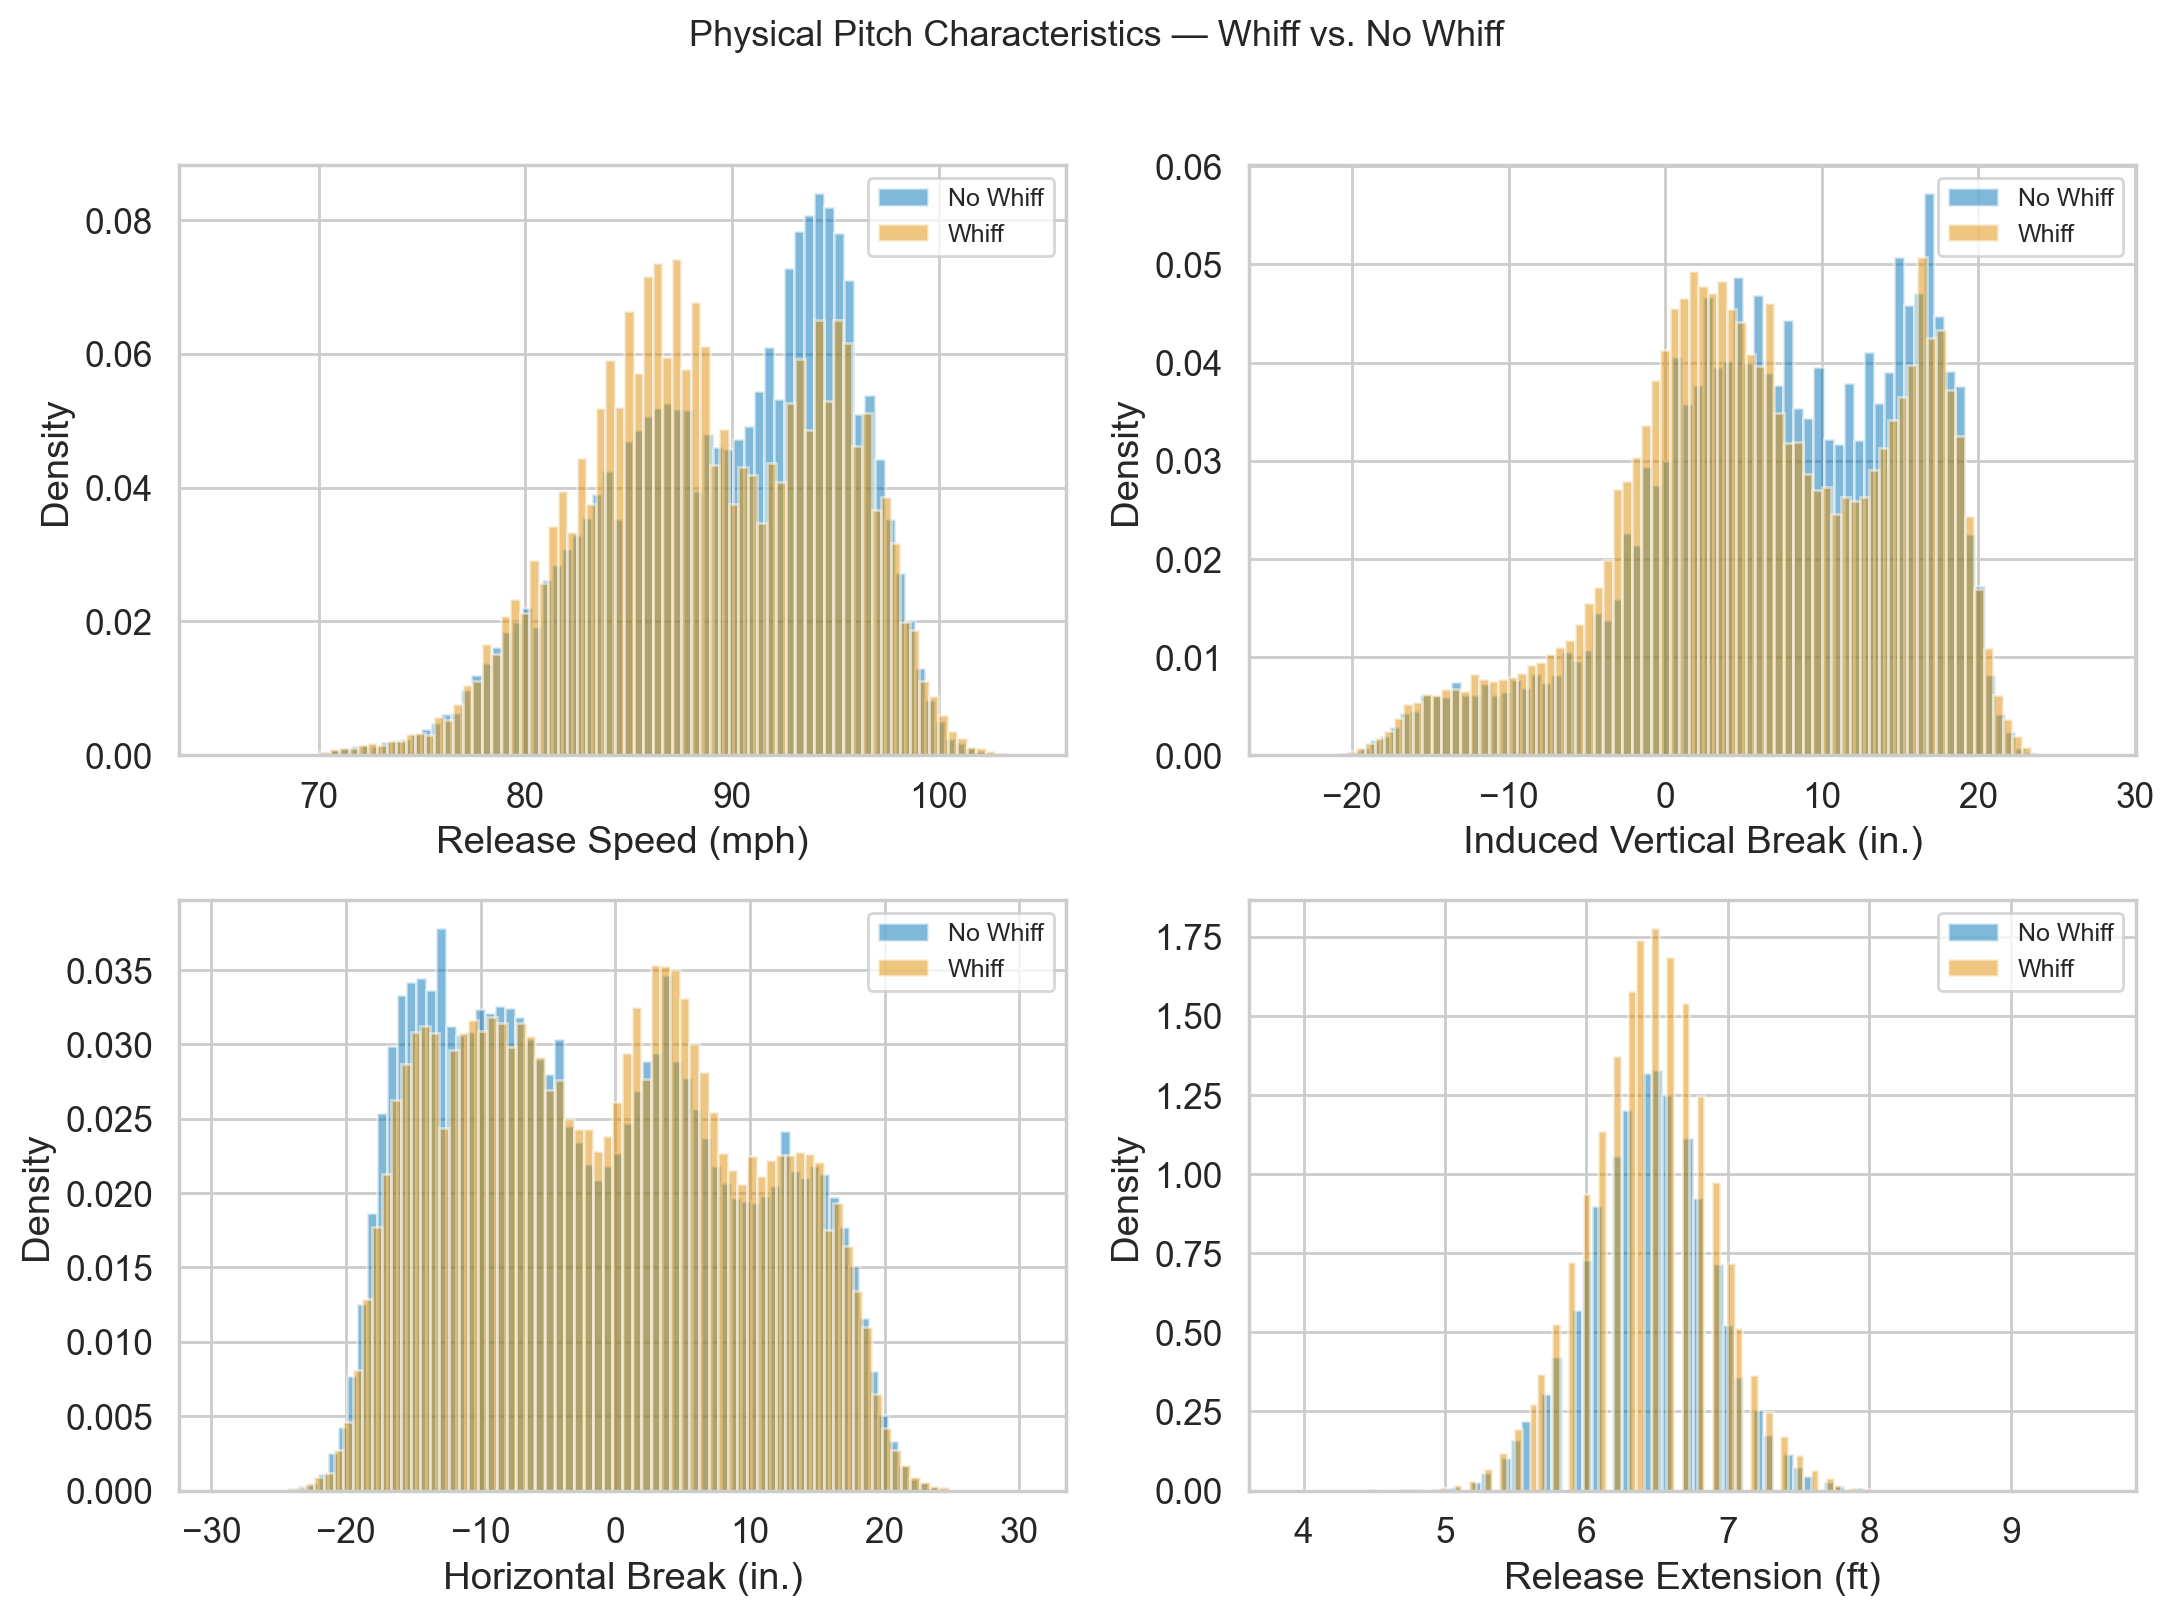
\includegraphics[width=0.9\textwidth]{figures/fig_physical_distributions.png}
    \caption{Density plots of physical pitch characteristics, stratified by outcome (whiff vs.\ no whiff). Differences across individual variables are subtle, motivating multivariate approaches.}
    \label{fig:phys_dist}
\end{figure}

\subsection{Pitch Sequencing Patterns}

A central hypothesis of this study is that pitch effectiveness depends on the preceding pitch.
Figure~\ref{fig:seq_heatmap} presents a heatmap of whiff rates organized by previous pitch type (rows) and current pitch type (columns).
Several noteworthy patterns are visible.

Splitters achieve the highest average whiff rate, and account for the three highest whiff rates on the heatmap: splitter $\rightarrow$ splitter (21.3\%), knuckle-curve $\rightarrow$ splitter (21.0\%), curveball $\rightarrow$ splitter (20.1\%). Other notable whiff rates include knuckle-curve $\rightarrow$ knuckle-curve (19.9\%), sinker $\rightarrow$ knuckle-curve (19.4\%), and slider $\rightarrow$ slider (19.3\%). Clearly, throwing the same pitch successively results in high whiff rates, suggesting that batters anticipate varied pitch sequences. However, they still struggle to adjust to consecutive breaking balls with substantially different movement paths. This is evident from the high whiff rates (16-20\%) across the board after sliders, sweepers, and curveballs. 

The three types of fastball (cutters, four-seam fastballs, and sinkers) exhibit the lowest whiff rates overall. Furthermore, sinkers display the lowest average whiff rate by a considerable margin, likely because they are thrown as management pitches. These are pitches designed for easy groundouts and weak contact, rather than swing-and-misses. Four-seam fastballs and cutters thrown after breaking balls tend to have relatively moderate whiff rates (10 - 13\%), suggesting that batters may choose not to swing on high-speed pitches after seeing off-speed pitches. Despite the low whiff rates on the three fastball types, follow-up pitches show moderate to high whiff rates (14-19\%), consistent with the pitch tunneling hypothesis, but not fully explaining it. When consecutive pitches appear similar out of the pitcher's hand but diverge in trajectory near the plate, the batter's ability to adjust is compromised.

These findings strongly motivate the inclusion of sequencing variables and pitch-type interaction terms in the logistic regression model defined by Equation~(\ref{eq:baseline}).

\begin{figure}[H]
    \centering
    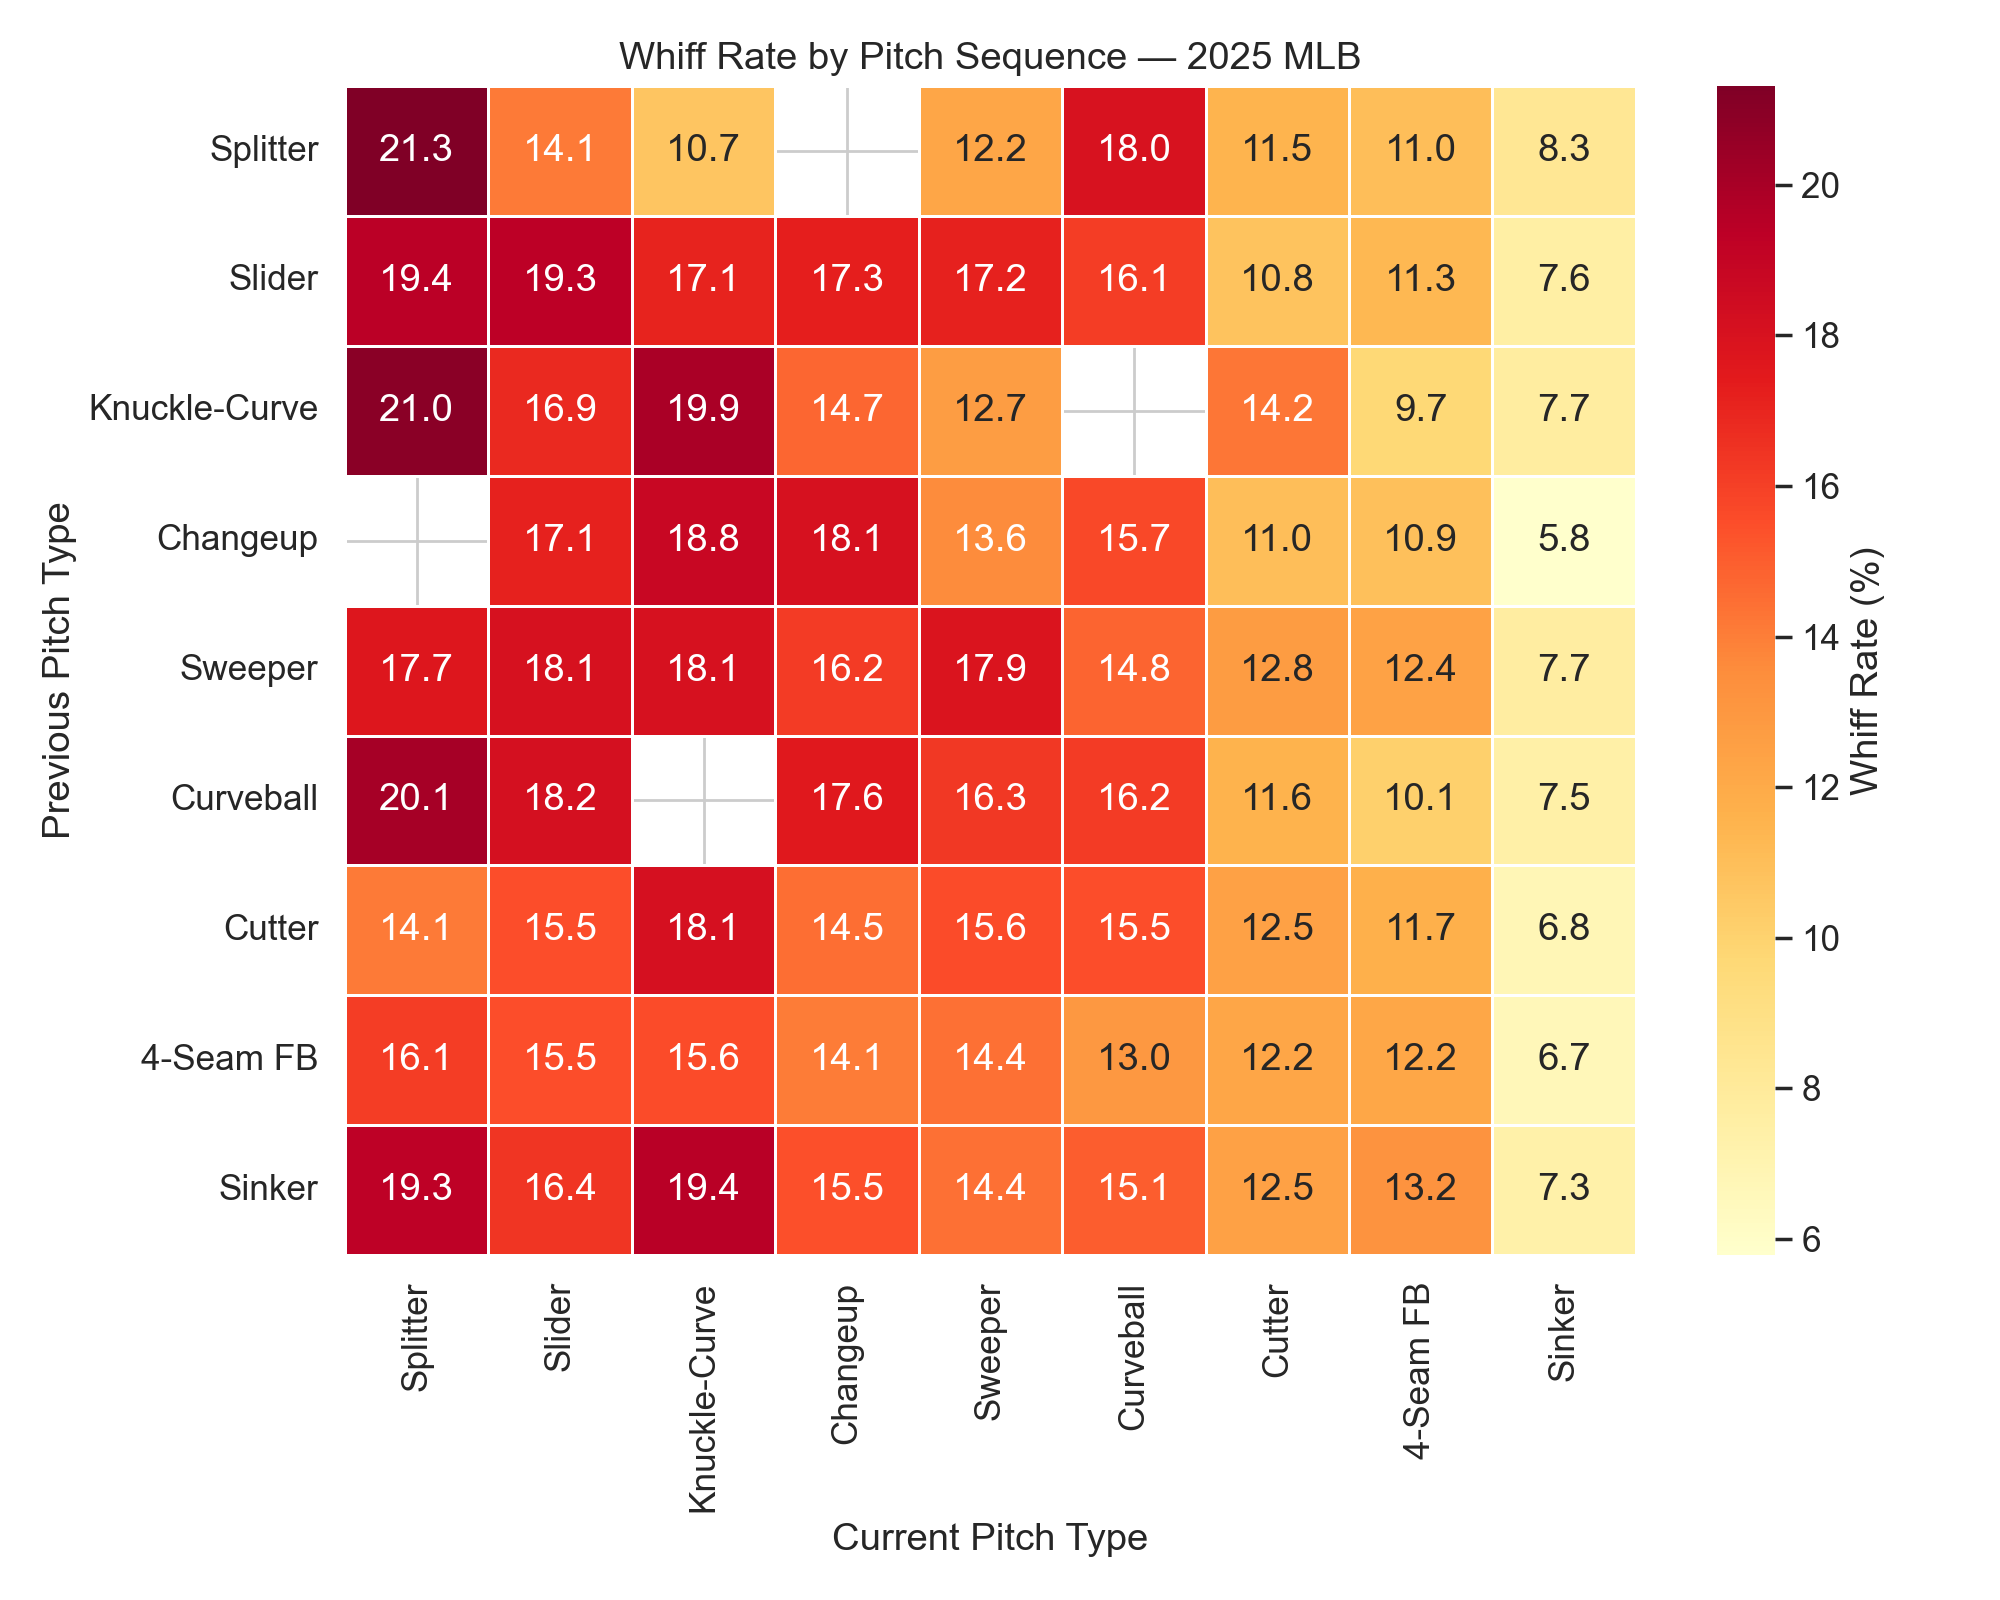
\includegraphics[width=0.85\textwidth]{figures/fig_sequence_heatmap.png}
    \caption{Heatmap of whiff rates by pitch sequence. Rows represent the previous pitch type; columns represent the current pitch type. Cells with fewer than 100 observations are excluded.}
    \label{fig:seq_heatmap}
\end{figure}

\subsection{Batter Heterogeneity}

To examine whether batter identity is an important source of variation, we compute per-batter whiff rates for all batters who faced at least 200 pitches during the season (\numBatters{} batters).
Figure~\ref{fig:batter_dist} shows the distribution of these batter-level whiff rates.
The distribution is approximately normal with an apparent spread: batter-level whiff rates range from roughly \batterLow\% to \batterHigh\%, illustrating the large degree of heterogeneity in contact ability across MLB hitters.
This variability confirms that batter identity is an important grouping factor and justifies the use of batter-level random intercepts in the planned GLMM.

\begin{figure}[H]
    \centering
    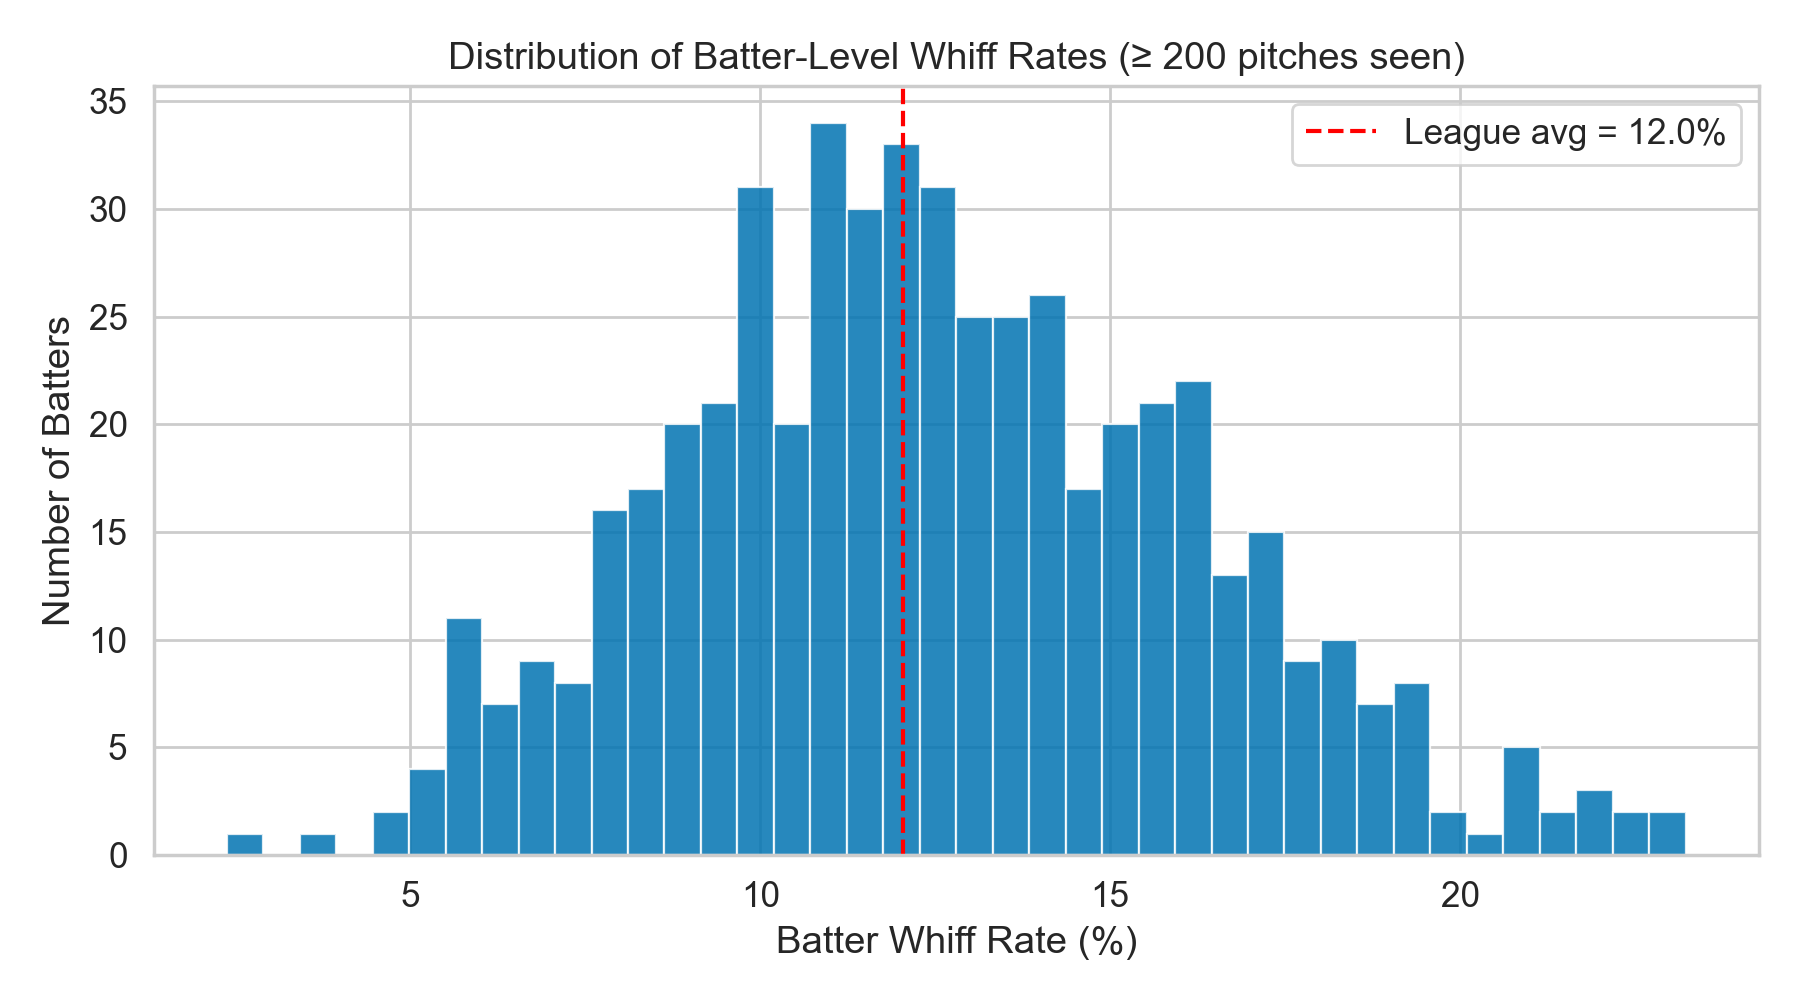
\includegraphics[width=0.8\textwidth]{figures/fig_batter_whiff_dist.png}
    \caption{Distribution of batter-level whiff rates (batters with $\geq 200$ pitches seen). The dashed red line marks the overall league whiff rate. Substantial heterogeneity motivates the use of batter random effects.}
    \label{fig:batter_dist}
\end{figure}

\subsection{Predictor Correlations}

Figure~\ref{fig:corr} shows the pairwise correlations among the continuous predictors and the binary whiff outcome.
The strongest relationship is between release speed and induced vertical break ($r = 0.72$). This makes sense because high-velocity fastballs tend to generate strong backspin, which leads to higher vertical break.
We wanted to take a deeper look at this with Variance Inflation Factors (VIFs) to ensure that multicollinearity did not affect the coefficient estimates.
Release speed and horizontal break are also negatively correlated ($r = -0.30$), which shows that slower breaking pitches tend to move more laterally.
Most importantly, none of the individual correlations with whiff exceed $|r| = 0.05$ in magnitude: release speed ($r = -0.05$), IVB ($r = -0.04$), HB ($r = 0.02$), and extension ($r = 0.01$).
This confirmed our initial theory that no single physical characteristic can decide swing-and-miss outcomes on its own, which meant we needed to look into a more comprehensive model, and more specifically, a combined model.

\begin{figure}[H]
    \centering
    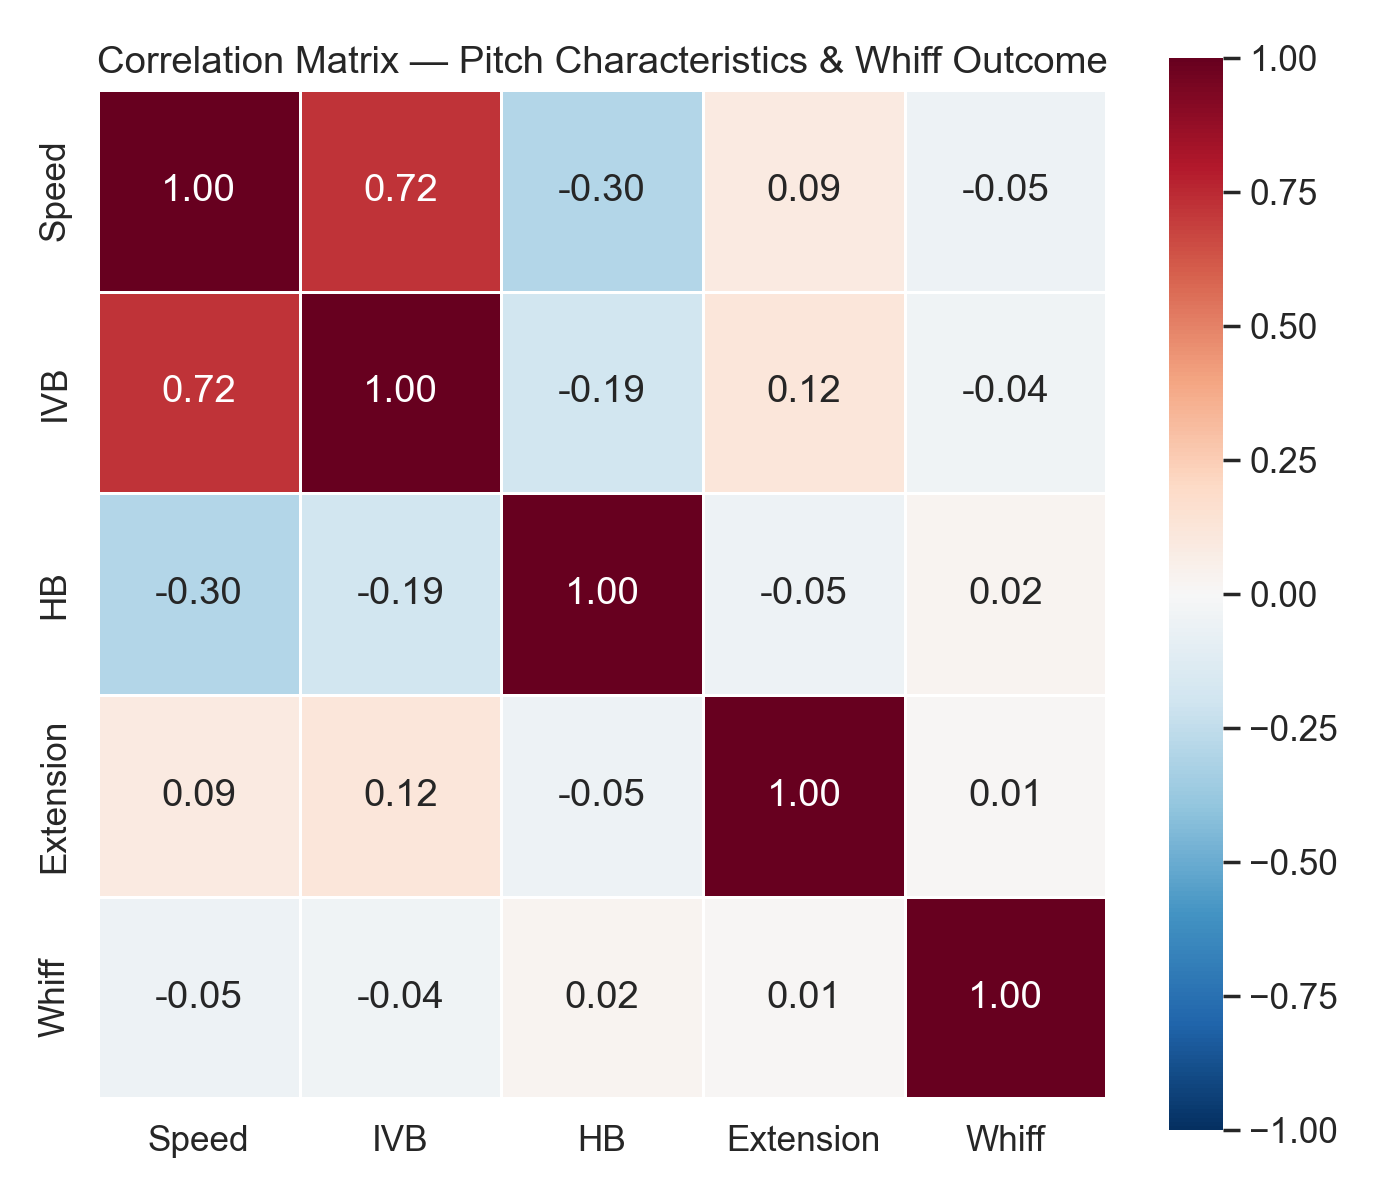
\includegraphics[width=0.6\textwidth]{figures/fig_correlation_matrix.png}
    \caption{Correlation matrix of continuous pitch characteristics and the binary whiff outcome. Correlations with whiff are small in magnitude, supporting the need for richer models.}
    \label{fig:corr}
\end{figure}

%%==============================================================
\section{Modeling Results}
%%==============================================================

\subsection{Baseline Logistic Regression}

We first fit the logistic regression from Equation~(\ref{eq:baseline}) using only physical characteristics. These are release speed, induced vertical break, horizontal break, and release extension.
For direct comparison with the richer fixed-effect models, we evaluate it on the same non-first-pitch subset used later for sequencing, which yields log-likelihood \seqLLBase{} and BIC \seqBICBase{}.
This reported baseline is the MLE reduced-model fit on non-first pitches, not the separate sklearn train/test implementation also present in the codebase.
The coefficient estimates in Figure~\ref{fig:base_coef} are small in magnitude even after standardizing the physical predictors, which is consistent with the weak marginal correlations observed in Figure~\ref{fig:corr}.
Release speed and induced vertical break both have negative coefficients, while horizontal break and extension have modest positive effects, but none of these effects is large enough to make the physical-only model competitive with the richer alternatives.
Substantively, the baseline model captures broad pitch-quality tendencies but still treats each pitch as an isolated event, so it leaves both sequence-dependent deception and batter-specific contact skill in the residual variation.

\begin{figure}[H]
    \centering
    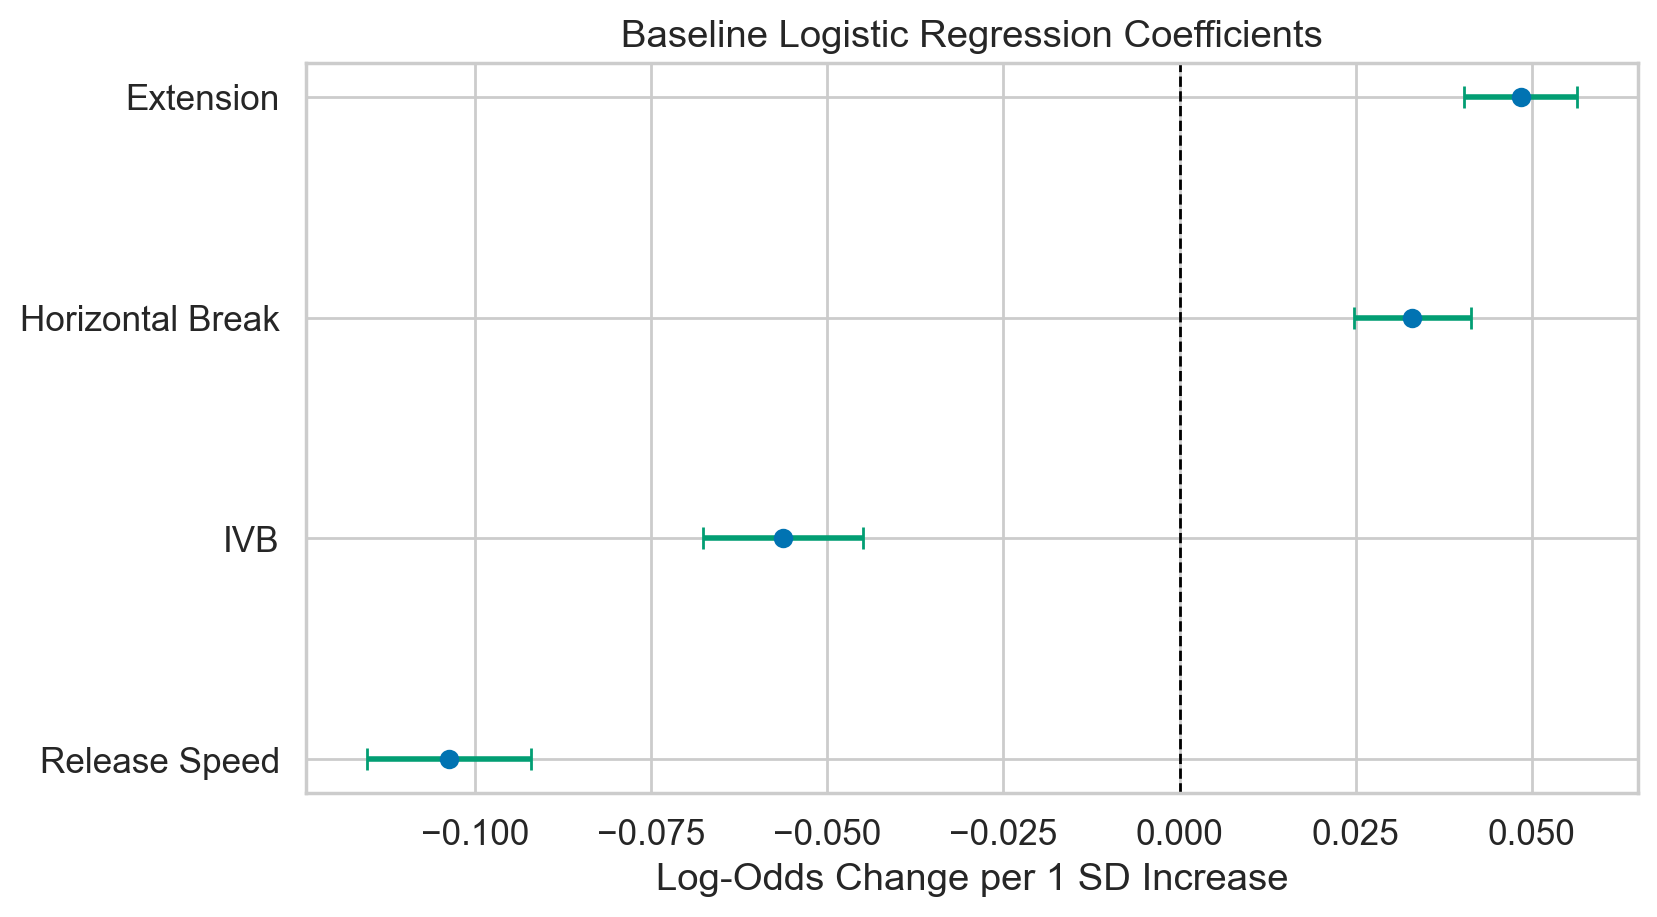
\includegraphics[width=0.72\textwidth]{figures/fig_baseline_coefficients.png}
    \caption{Baseline logistic-regression coefficient estimates with 95\% confidence intervals. Predictors are standardized, so each coefficient represents the change in log-odds of a whiff for a one-standard-deviation increase in the corresponding physical variable.}
    \label{fig:base_coef}
\end{figure}

\subsection{Sequencing Model}

We next extend the baseline model with features for the previous pitch type, previous pitch zone, previous pitch outcome, and current$\times$previous pitch-type interaction effects.
Relative to the baseline model fit to the same observations, the sequencing model increases the log-likelihood from \seqLLBase{} to \seqLLSeq{}.
The likelihood-ratio statistic is \seqLRStat{} on \seqLRDf{} degrees of freedom with a p-value of \seqLRPval{}, confirming the sequencing terms are jointly significant.
The BIC also improves from \seqBICBase{} to \seqBICSeq{} (\(\Delta\)BIC = \seqDeltaBIC{}), indicating the fit gain is substantial enough to justify the additional model complexity.
Figure~\ref{fig:seq_terms} presents the largest pitch-sequence interaction terms from this model.
The strongest positive effects all occur when a four-seam fastball is followed by a breaking or off-speed pitch, especially four-seam fastball $\rightarrow$ knuckle-curve, splitter, sweeper, and slider.
The one large negative interaction in Figure~\ref{fig:seq_terms} is four-seam fastball $\rightarrow$ sinker, which is consistent with sinkers functioning more as contact-management pitches than swing-and-miss pitches.
Taken together, these results support the sequencing hypothesis; whiff probability depends not just on what pitch is thrown, but on what the batter just saw.

\begin{figure}[H]
    \centering
    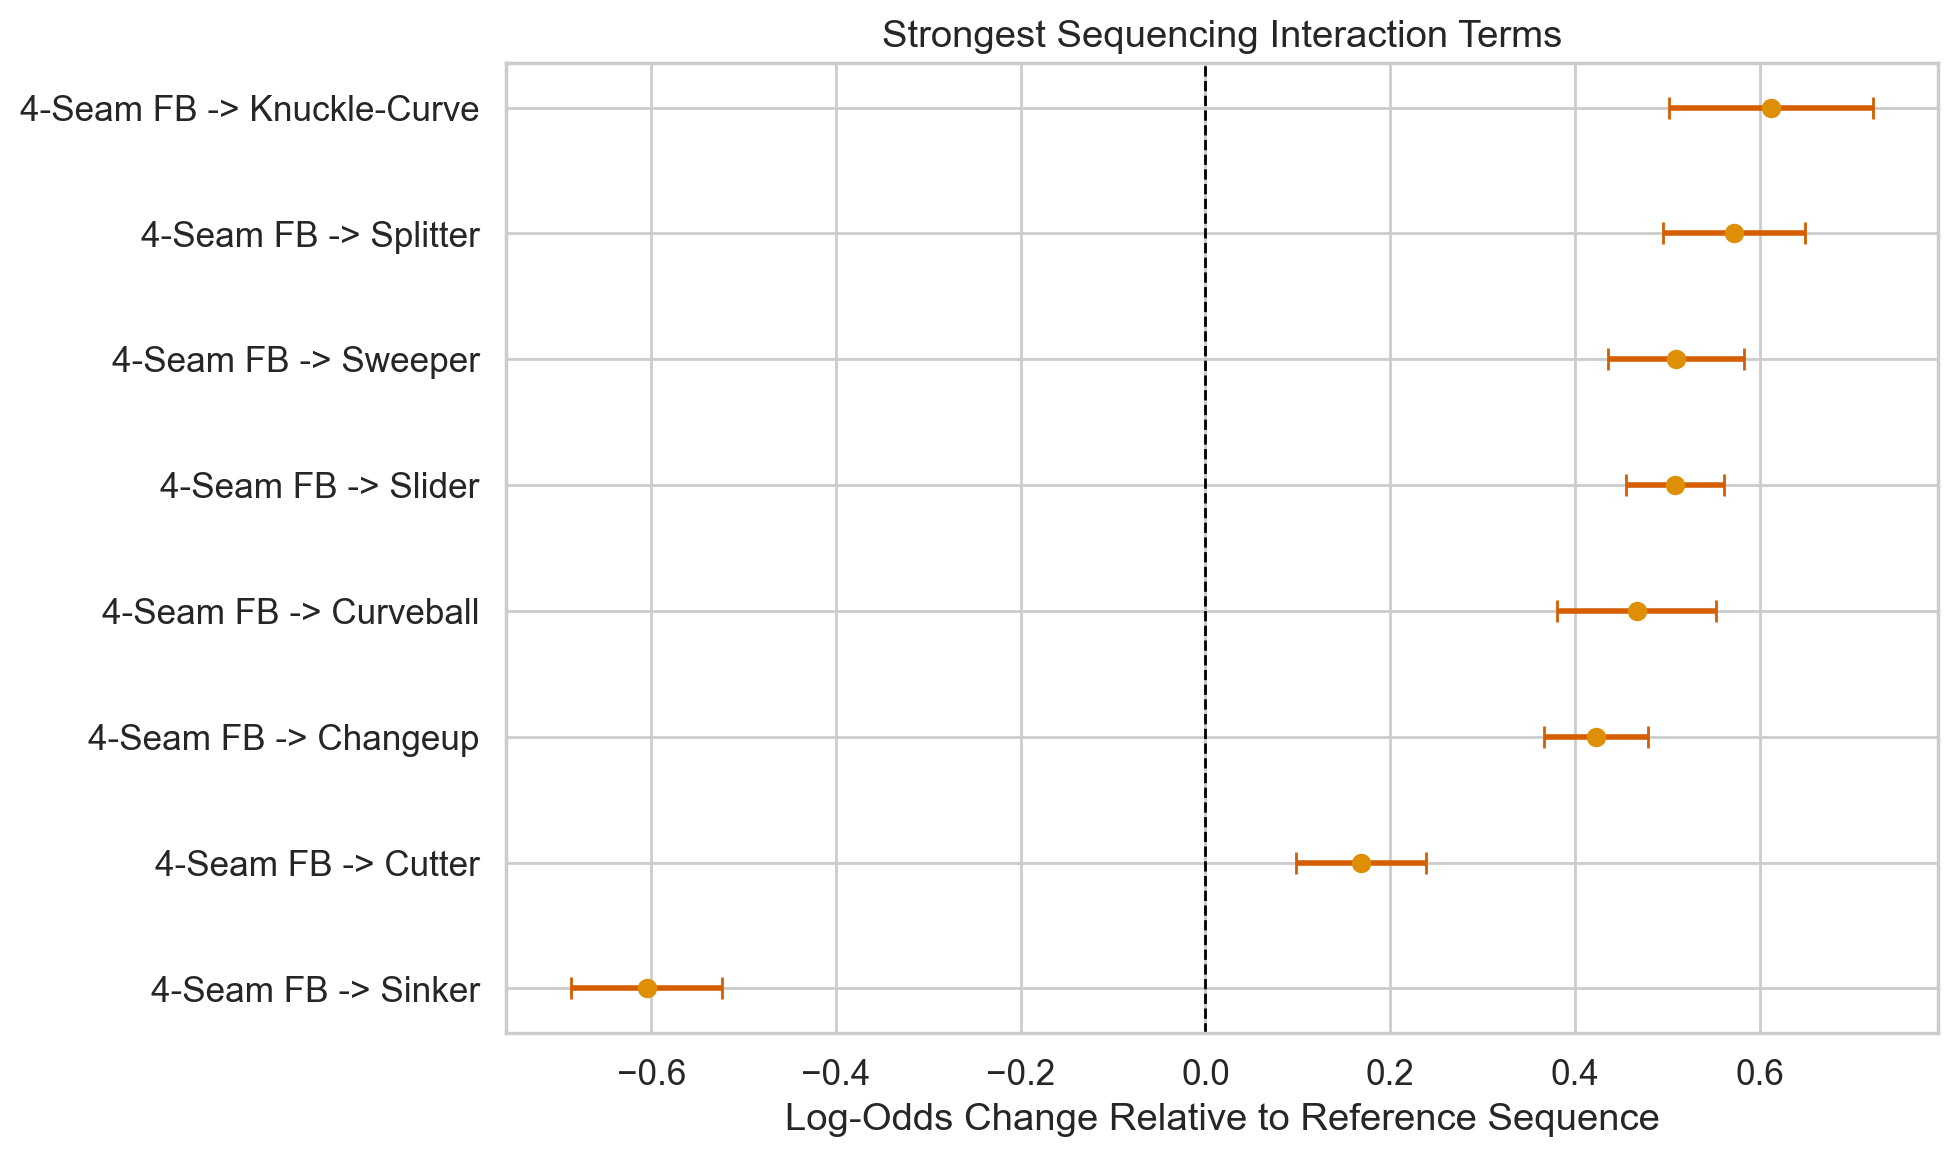
\includegraphics[width=0.82\textwidth]{figures/fig_sequencing_terms.png}
    \caption{Significant sequencing interaction terms ($p < 0.05$, pitch-pair sequences with $n \ge 100$ observations). Positive coefficients indicate pitch sequences that increase whiff probability relative to the reference sequence, while negative coefficients indicate sequences that reduce it.}
    \label{fig:seq_terms}
\end{figure}

\subsection{GLMM with Batter Random Intercepts}

We next fit a standalone GLMM that focuses on batter heterogeneity directly by adding a batter-level random intercept to the logistic model.
In the notebook implementation, this model is estimated with \texttt{BinomialBayesMixedGLM} using the same sequencing-style fixed-effect structure and a random intercept for batter.
In order to be within computational limits, the GLMM is fit on a random subsample of \glmmObs{} pitches from the sequencing dataset, spanning \glmmBatters{} batters and \glmmFixed{} fixed-effect terms.
The estimated standard deviation of the batter random intercept is \glmmSigma{} (variance \glmmSigmaSq{}), which implies an intra-class correlation of \glmmICC\%.
On the latent log-odds scale, this means that a nontrivial share of the remaining variation in whiff probability lies between batters rather than within batters across pitches.
That result matters because it shows that batter identity is not just a noisy grouping factor: even after controlling for pitch physics and pitch context, hitters still differ systematically in baseline swing-and-miss tendency.
Because this GLMM is fit via variational Bayes on a subsample for tractability, we treat it primarily as evidence about the magnitude of batter-level heterogeneity rather than place it in the full-sample BIC comparison used for the fixed-effect and combined models.

\subsection{Combined Model}

Finally, the combined model adds batter-specific random intercepts to the sequencing model. This allows each hitter to have a different baseline tendency to swing and miss while the model still estimates the same pitch-level and sequencing effects for the full dataset.
The model is fit as a logistic mixed model with one random intercept for each of the 673 batters appearing in the non-first-pitch modeling subset.
Its log-likelihood is \combLogLik{} and its BIC is \combBIC{}, improving on both the baseline and sequencing-only fits.
Relative to the sequencing model, the combined model lowers BIC by 4{,}146.22 and increases log-likelihood by roughly 2{,}047. This shows that batter heterogeneity still matters even after sequencing is included.
Figure~\ref{fig:model_compare} shows the fit comparison across the three models estimated on the common full-sample likelihood framework. Figure~\ref{fig:combined_re} plots the estimated batter random intercepts from the combined model.
The estimated random-intercept standard deviation is \combRandSD{}, which confirms that batter-level heterogeneity remains substantial after controlling for pitch characteristics and sequencing.
This result matters because some hitters maintain low whiff propensities in nearly every context, while others remain vulnerable even after accounting for the types and order of pitches they see.
Taken together, the combined model provides the clearest decomposition of whiff probability into pitch-quality effects, sequence effects, and batter-specific contact skill.

\begin{figure}[H]
    \centering
    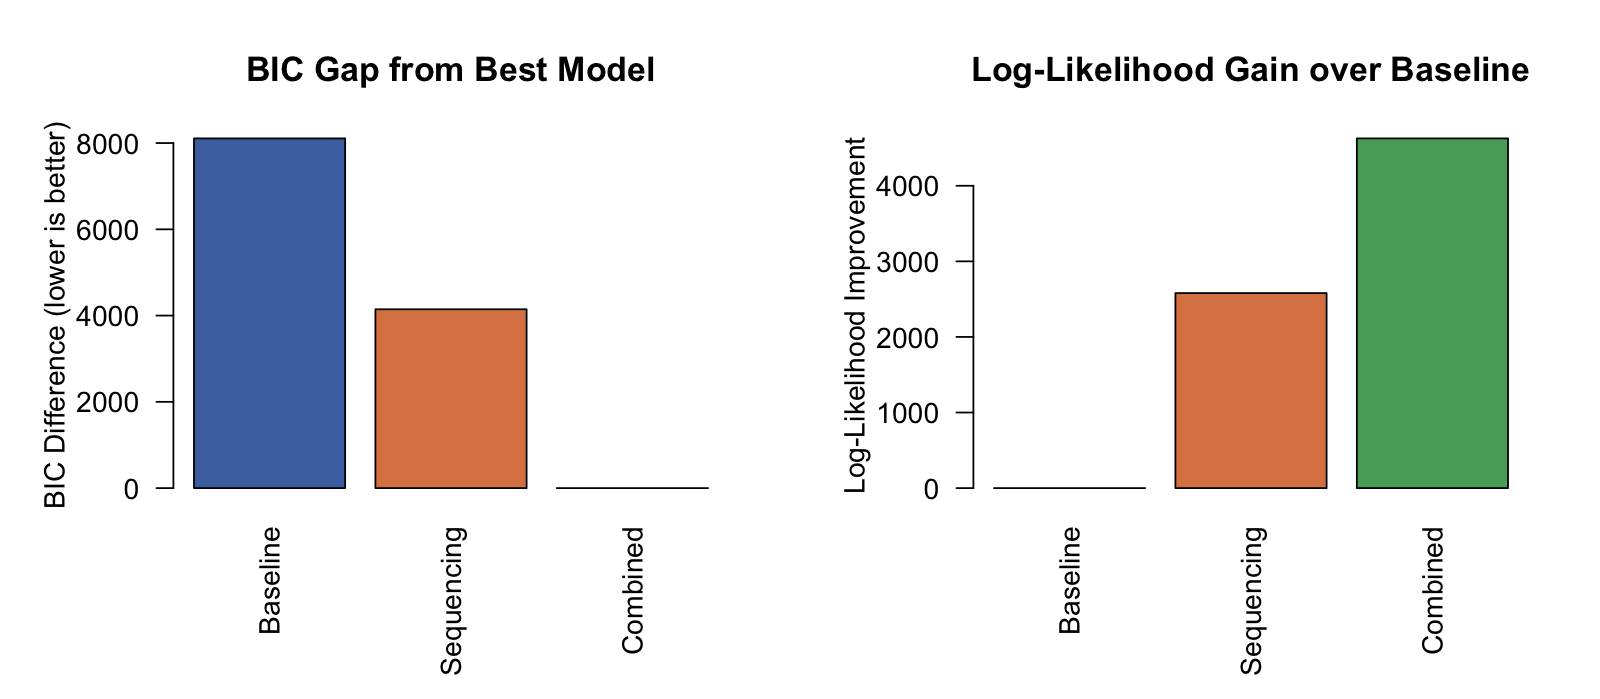
\includegraphics[width=0.9\textwidth]{figures/fig_model_comparison.png}
    \caption{Model comparison across the baseline logistic regression, the sequencing model, and the combined model. The left panel shows each model's BIC gap from the best-fitting specification, while the right panel shows the gain in log-likelihood relative to the baseline model. The standalone GLMM is omitted because it was fit with a different estimator on a subsample.}
    \label{fig:model_compare}
\end{figure}

\begin{figure}[H]
    \centering
    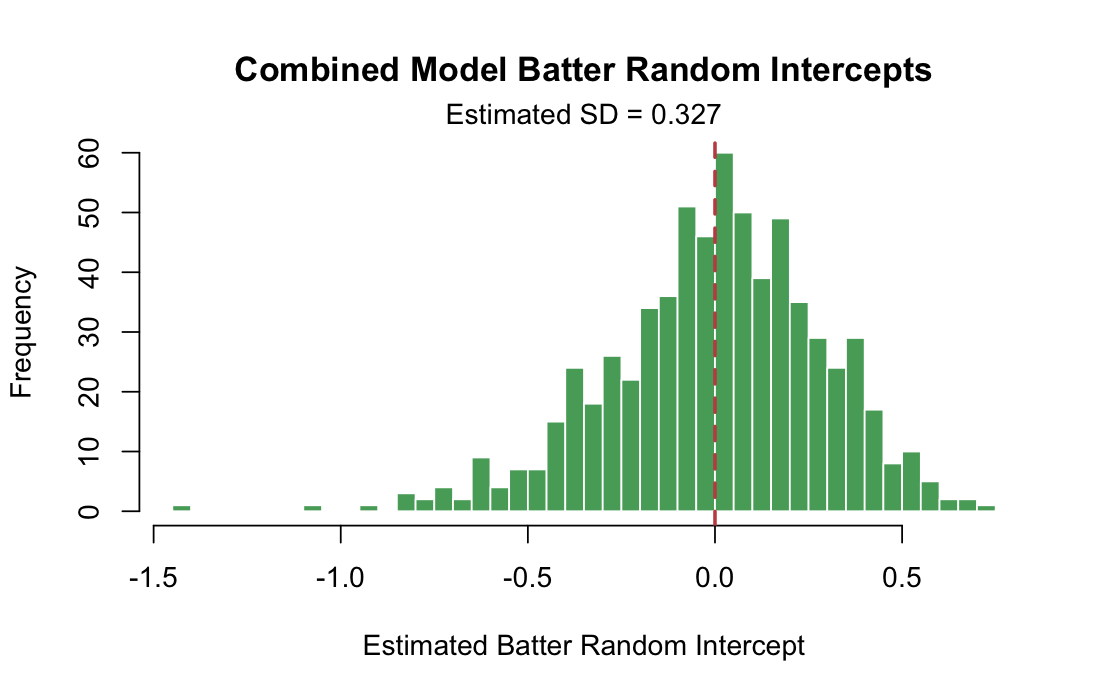
\includegraphics[width=0.75\textwidth]{figures/fig_combined_batter_effects.png}
    \caption{Distribution of batter random intercepts from the combined model. The spread of the fitted intercepts indicates meaningful batter-to-batter differences in baseline whiff tendency even after controlling for pitch characteristics and sequencing.}
    \label{fig:combined_re}
\end{figure}

%%==============================================================
\section{Conclusion}
%%==============================================================

The central finding of this analysis is that physical pitch characteristics are informative but incomplete on their own.
The baseline logistic regression provides a useful benchmark, yet the sequencing model shows that much of the remaining explanatory power lies in pitch context. The previous pitch type, previous result, and specific previous $\rightarrow$ current pitch combinations all carry meaningful information about whether a batter will swing and miss.
The standalone GLMM then shows that batter-level heterogeneity is present but modest even after introducing those pitch-context covariates, with the estimated ICC of \glmmICC\% suggesting batter identity explains only a small share of whiff variation.
Once batter-specific random intercepts are added directly to the sequencing model, the final combined model captures that additional source of systematic variation and becomes the best-fitting model by a substantial margin.

These results are consistent with the baseball interpretation developed in the exploratory analysis.
Pitchers do not generate whiffs solely by throwing hard or by maximizing raw movement; they also generate whiffs by choosing pitch orders that distort timing and by exploiting batter-specific weaknesses.
From a statistical standpoint, that means the most useful model is the one that jointly accounts for pitch-level characteristics, sequential context, and batter heterogeneity.
This combined approach gives the best fit among the directly comparable models, and yields the most realistic picture of how swing-and-miss outcomes arise over the course of a plate appearance.


%% BIBLIOGRAPHY
%%==============================================================
\newpage
\bibliographystyle{chicago}
\bibliography{FinalReportRef}

\newpage
\section*{Code Repository}
The main data analysis code is provided in the project repository:
\begin{center}
\url{https://github.com/hdav3228/STAT482}
\end{center}
The repository includes the Python exploratory analysis, logistic regression
models, notebook-based GLMM workflow, and combined mixed-effects model code.

\end{document}
